Tritium is the third natural isotope of the hydrogen. IUPAC has declared that, while tritium is usually designed by the symbol T, it is not recommend. The nomenclature which is currently accepted sets that it should be symbolized as $\ce{^{3}H}$. 

The first natural isotope of hydrogen, whose name is protio, has only one proton in its nucleus and it is the most abundant (approximately $75\%$ of the visible matter of the universe). Its natural abundance among the hydrogen isotopes is more than $99.985\%$. The second natural isotope of hydrogen, deuterium, has one proton and one neutrons in its nucleus and its natural aboundance among the hydrogen isotopes is between $2.6 \cdotp 10^{-3}\%$ and $1.8 \cdotp 10^{-2}\%$. The most usually situation is to find the lower percent for the gas hydrogen and the higher percent in the seawater. Finally the third natural isotope of hydrogen, the tritium, has one proton and two neutrons in its nucleus. It is an unstable isotpe, that's, a radioactive isotpe which we can find in little quantities in the environmental. All this valuers are resumed in the table \ref{PropHIsot}. In the \ref{fig:HydrogenIsotopes} figure we can see the representation of this three first isotopes of the hydrogen which are the only natural isotopoes of hydrogen in the environmental.

\begin{table}[htbp]
\begin{center}
\begin{tabular}{|l|l|l|l|l|}
\hline
Physical & Common & Name & Natural Abundance (\%) & Mass (mass units) \\
\hline \hline \hline
$\ce{\ce{^{1}_{1}H}}$ & H & Protium & 99.985 & 1.007825 \\ \hline
$\ce{\ce{^{2}_{1}H}}$ & D & Deuterium & $\approx$ 0.015 & 2.01400 \\ \hline
$\ce{\ce{^{1}_{1}H}}$ & T & Tritium & $1 \cdot 10^{-18}$ & 3.01605\\ \hline
\end{tabular}
\caption{Hydrogen isotopes (hydrogen, deuterium, tritium)~\cite{documento manipulación segura tritio}}
\label{PropHIsot}
\end{center}
\end{table}

\begin{figure}[hbtp]
\includegraphics[scale=0.6]{Hydrogen_isotopes.png}
\centering
\caption{Three first isotopes of the hydrogen (hydrogen, deuterium, tritium)~\cite{dondesea}\label{fig:HydrogenIsotopes}}
\end{figure}

There are other heavier hydrogen isotopes which not exist in nature. Nowadays we know that there's exist from $\ce{^{4}_{1}H}$ until $\ce{^{7}_{1}H}$. All these heavier isotopes than tritium only exist in the laboratories and they are unstable isotopes whose half life time is less than a zeptosecond ($10^{-21}$). Among this heavier isotopes, the most stable is $\ce{^{5}_{1}H}$ ($T_{1/2} > 9.1\cdot 10^{-22}~\second$)\cite{wikipediaAnexoIsotoposDeHidrogeno} and the less stable is $\ce{^{7}_{1}H}$ ($T_{1/2} = 2.3 \cdot 10^{-23} ~\second$)\cite{wikipediaAnexoIsotoposDeHidrogeno}. 

The $\ce{^{4}_{1}H}$ is produced by bombardment of tritium atoms with high-speed deuterium nucleis \cite{asdfasd} where the tritium nuclei capture one neutron to deuterium nuclei \cite{asdfasdf}. The $\ce{^{5}_{1}H}$ is produced by bombardment of tritium atoms with high-speed tritium nucleis where the tritium nuclei capture two neutrons to other tritium nuclei. \cite{asdfasd}. The $\ce{^{7}_{1}H}$ is produced by bombardment of hydrogen atoms with a helium isotope, $\ce{^{8}_{2}He}$ nucleis where the helium neutros is given to the hydrogen nuclei. \cite{asdfasd}. 

These isotopes decay by neutron emission through the following nuclear reactions:

\begin{equation}
\ce{^{4}_{1}H} \rightarrow \ce{^{3}_{1}H} + \ce{n}
\label{H4}
\end{equation}

\begin{equation}
\ce{^{5}_{1}H} \rightarrow \ce{^{4}_{1}H} + \ce{n}
\label{H5}
\end{equation}

\begin{equation}
\ce{^{6}_{1}H} \rightarrow \ce{^{3}_{1}H} + 3 \cdot \ce{n}
\label{H6}
\end{equation}

\begin{equation}
\ce{^{6}_{1}H} \rightarrow \ce{^{4}_{2}He} + 2 \cdot \ce{n}
\label{H62}
\end{equation}

Tritium was first time produced in $1934$ from neutron capture of deuterium, $\ce{^{2}_{1}H}$, by Ernest Rutherford, Mark Oliphant and Paul Harteck \cite{TritiumDiscovery} but they couldn't isolate it. First time when tritium was isolated was in 1939 by Luis Walter Alvarez and Robert Cornog \cite{TritiumIsolate}, who saw that tritium was a radiactive element. 

Tritium is a radiactive isotope which we can find in the enviromental because it is normally produced through the interaction of cosmics rays and gaseous elements of the upper atmosphere, for example, through the following nuclear reaction:

\begin{equation}
\ce{^{14}_{7}N} + \ce{n} \rightarrow \ce{^{3}_{1}H} +  \ce{^{12}_{6}C}
\label{H62}
\end{equation}

Then tritium becomes water and reaches the earth's surface as rain with an estimated produccion rate of $4\cdot 10^6$ Ci/yr. 

It can be also producen artificially by means of commercial producers of radioluminicent and neutron generator devices ($1 \cdot 10^6$ Ci/yr), atmospheric nuclear test explosions between 1945 and 1975 ($8 \cdot 10^9$ Ci/yr/GW), nuclear power and defense industries ($1-2 \cdot 10^6$ Ci/yr). 

It is usully also produced artificialy in several laboratories by bombardment of lithium, boron or nitrogen targets with neutrons free as you can see in the follow nuclear reactions:

PONER LA GRAFICA DE CANTIDAD DE TRITIO NATURAL HOY EN DIA DE LA TESIS QUE HABÍA EN EL LARAM.

\begin{equation}
\ce{^{6}_{3}Li} + \ce{n} \rightarrow \ce{^{3}_{1}H} + \ce{^{4}_{2}He}
\label{capneuLi6}
\end{equation}

\begin{equation}
\ce{^{7}_{3}Li} + \ce{n} \rightarrow \ce{^{3}_{1}H} + \ce{^{4}_{2}He} + \ce{n}
\label{capneuLi7}
\end{equation}

\begin{equation}
\ce{^{10}_{5}B} + \ce{n} \rightarrow \ce{^{3}_{1}H} + 2 \cdot{} \ce{^{4}_{2}He}
\label{capneuB10}
\end{equation}

\begin{equation}
\ce{^{11}_{5}B} + \ce{n} \rightarrow \ce{^{3}_{1}H} + 2 \cdot{} \ce{^{4}_{2}He} + n
\label{capneuB11}
\end{equation}

\begin{equation}
\ce{^{14}_{7}Ni} + \ce{n} \rightarrow \ce{^{3}_{1}H} + \ce{^{12}_{6}C}~~~[\ref{librooo}]
\label{capneuN14}
\end{equation}
%$\eqref{capneuLi6}$ para referenciar ecuaciones

There are two more nuclear reaction with which we can produce tritium. It is the next:

\begin{equation}
\ce{^{1}H} + 2 \cdot{} \ce{n} \rightarrow \ce{^{3}T}
\label{doblecapneuH}
\end{equation}

\begin{equation}
\ce{^{2}D} + \ce{n} \rightarrow \ce{^{3}T}
\label{capneuD}
\end{equation}

In the environmental both reactions are negligible ways to produce tritium because we have few quantity of deuterium and few neutrons with enough energy for producing this nuclear reaction. However it is one of the channel with the highest tritium production in a nuclear power plant, which is the place where the detector we will be installed.

INTENTAR BUSCAR LA ENERGÍA DE LOS NEUTRONES A LA CUAL PUEDE PRODUCIRSE ESTA REACION!!!

It happen because in a nuclear power plant we have a big quantity of neutrons with enough energy ($10^{14} ~\ce{n} \, \cm^{-2} \second^{-1}$ as we have said in the chapter \ref{chap:GeneralIntroduction}, section \ref{sec:Introduction}). Furthermore we have a lot of deuterium in their cooling system.

In fact, the production of tritium is more likely in nuclear power plants where heavy water ($\ce{D_2 O}$) or semi-heavy water ($\ce{H}\ce{D}\ce{O}$) is used as a refrigerant because there we have a lot of deuterium as a part of their molecules. When nuclear power plant use normal water as a refrigerant ($\ce{H_2 O}$) this production channel is not so important since the natural concentration of deuterium is very low. This concentration is between $0.0026\%$ and $0.0184\%$ in population (a little bit large percentage in mass because deuterioum is more heavy than hydrogen). In the sea water it is more or less $0.015\%$ and less for gas.

We have to take into account that this concentration in modified in a nuclear power plants that use normal water as a refrigerant because, although they use water from the sea or from the river, we have a lot of neutrons in these facilities so the quantity of deuterium will be increased due to the neutron capture of the hydrogen:

\begin{equation}
\ce{^{1}H} + \ce{n} \rightarrow \ce{^{2}D}
\label{capneuH}
\end{equation} 

And tritium can be formed from this deuterium with the reaction \eqref{capneuD}, previously mentioned or directly like a doble neutron capture \eqref{doblecapneuH}.

We have to take into account that we also has tritium like a gas and tritium water can be also formed in a nuclear reactor from this tritium gas. In the table \ref{GasMolecules} you can see the possible combinations of gas molecules between hydrogen ($\ce{H}$), deuterium ($\ce{D}$)  and tritium ($\ce{T}$) and their boiling points which we can find in a nuclear reactor are:

\begin{table}[htbp]
\begin{center}
\begin{tabular}{|l|l|l|}
\hline
Molecule & Boiling point (for gases) ($\kelvin$) & oxidation form\\
\hline \hline \hline
$\ce{H_2}$ & 20.39 & $\ce{H_2 O}$ \\ \hline
$\ce{HD}$ & 22.14 & $\ce{HDO}$ \\ \hline
$\ce{HT}$ & 22.92 & $\ce{HTO}$ \\ \hline
$\ce{D_2}$ & 23.66 & $\ce{D_2 O}$ \\ \hline
$\ce{DT}$ & 24.38 & $\ce{DTO}$ \\ \hline
$\ce{T_2}$ & 25.04 & $\ce{T_2 O}$ \\ \hline
\end{tabular}
\caption{Gas molecules in a nuclear reactor and their boiling points}
\label{GasMolecules}
\end{center}
\end{table} 

COMPUESTOS DEUTERADOS Y TRITIADOS PREESNTAN LA MISMAS PORPIEDADES QUIMICAS PERO ALGUNAS DIFERENCIAS ISOTRÓPICAS -> TABLA 2 DE MANIPULACIÓN DEL TRITIO

LAS PRIPIEDADES BIOLOGICAS DEL TRITIO SE CONOCEN MUY BIEN. PUnto 3 de manipulación seguro del tritio.

Tritio gaseoso en aire inalado muy poco eficiente, conversión del 0.003 o 0.005 poricento. En la piel practicamente nulo

agua tritiada, respirada porque esta en el aire o bebida, presenta una absorcion del 99\%. Para la piel también es muy alta. En 2 horas se distribuiye por tod oel cuerpo y la retención es caracteristica del agua.

En metales se sabe poco. Dependiendo del metal ocurre una cosa u otra.

VIDA MEDIA DEL TRITIPO 9.5 DIAS +-50\%



 Estos diversos compuestos tritiados tienen una amplia gama de propiedades metabólicas en humanos bajo condiciones de exposición similares. Por ejemplo, el gas de tritio inhalado solo se incorpora ligeramente al cuerpo durante la exposición, y el resto se elimina rápidamente (por exhalación) después de la exposición. Por otro lado, el vapor de agua tritiado se absorbe y retiene fácilmente en el agua del cuerpo.

There are small chemical differences between tritium and the other natural isotopes of the hydrogen, something which doesn't happen with other elements and this is because they have a large relative difference in their molecular masses. It doesn't happen with other elements because they are heavier so the difference in their relative mass when we introduce one or more neutrons is smaller. It affect in several things such as different boiling point (as you can see), which is higger for larger masses. It also happen for heavy water or super-heavy water than normal water.

In the table \ref{GasMolecules} we find the oxidation form of this elements. The most common form of this elements (apart of $\ce{H_2 O}$) is $\ce{HTO}$. This oxidation is formed when this gas molecules are in contacte with oxigen or water vapor according to available information from Los Alamos National Laboratory (LANL) \ref{manipulación del tritio}.   It can be formed for oxidation or exchange as you can see in the folowing nuclear reactions:

\begin{equation}
\begin{split}
& Oxidation: \\
& 2\cdot{}\ce{HT} + \ce{O_2} \rightarrow 2 \cdot{} \ce{HTO}\\
& 2\cdot{}\ce{T_2} + \ce{O_2} \rightarrow 2 \cdot{} \ce{T_2 O}
\label{oxidation}
\end{split}
\end{equation}

\begin{equation}
\begin{split}
& Exchange: \\
& \ce{HT} + \ce{H_2 O} \rightarrow \ce{H_2} + \ce{HTO}\\
& \ce{T_2} + \ce{H_2 O} \rightarrow \ce{HT} + \ce{HTO}\\
\label{exchange}
\end{split}
\end{equation}

These reactions can be increased by radiation (from near tritium until high concentratrions) or heat (both conditions are included inside of a nuclear reactor). They can be also increased  with some metal catalysts, specially palladium or platinum. 

We have to take into account that tritium can performe all the chemical reactions with the hydrogen can do, some times with higher rate if the tritium concentration is high enough to catalyze the reaction. From our point of view one of the most important reactions are when a molecule exchanges one or two  of their hydrogen atoms for a tritium atom since in this case we have tritium water in the cooling system. This reaction has to be catalyzed because, on the contrary, it is too slow because the hydrogen is strongly bonded. 

Tritium is a radioactive element whose half-life time is $T_{1/2}= 12.32$ years. It decays exclusively through $\beta$ radiation, it means that it don't have other type of decays like $\gamma$ decays so tritium don't has almost radiotoxicity. In this decay, one out of their two neutrons of their nucleus is transformed in a proton plus electron and electron antineutrino according to the following equation:

\begin{equation}
\ce{n} \longrightarrow \ce{p^+}  + \ce{e^-}  + \ce{\overline{\nu}_e}
\label{BetaDecay}
\end{equation}

Then the nucleus of the tritium son in this reaction has two protons and one neutron so it is a helium isotope, $\ce{^{3}_{2}He}$. $\ce{^{3}_{2}He}$ and $\ce{^{4}_{2}He}$ are the only stable helium isotopes in the environmental which we know but there are more unstable isotopes, from $\ce{^{2}_{2}He}$ up to $\ce{^{8}_{2}He}$ which is produced only in laboratories. $\ce{^{3}_{2}He}$ and $\ce{^{4}_{2}He}$ are normally used for cooling systems since we can arrive up to less than 1 Kelvin with they.

Therefore, the nuclear reaction which descript the $\beta^-$ decay of the tritium is:

\begin{equation}
\ce{^{3}T} \longrightarrow \ce{^{3}He}  + \ce{e^-}  + \ce{\overline{\nu}_e}
\label{TritiumDecay}
\end{equation}

In the Figure \ref{fig:TritiumDecay} there is a scheme of tritium energy levels where we can check that the only way of tritium decay is a $\beta^{-}$ decay until $\ce{^{3}_{2}He}$.

\begin{figure}
 \centering
  \subfloat[Scheme of the energy levels of tritium]{
   \label{fig:Energy levels}
    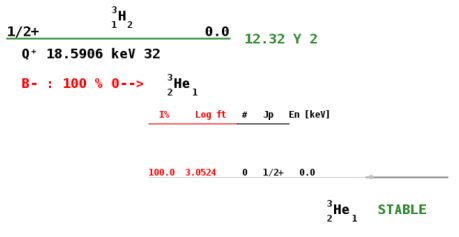
\includegraphics[width=0.5\textwidth]{esquema_niveles_energeticos.png}}
  \subfloat[Graphic representation of tritium decay]{
   \label{fig:GraphicDesintegration}
    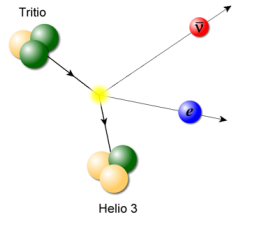
\includegraphics[width=0.5\textwidth]{representacion_desintegracion.png}}
 \caption{Tritium decay}
 \label{fig:TritiumDecay}
\end{figure}

The energy that is released in this nuclear reaccion is constant $18.6~\keV$ but it is divided between the products of this reaccion. Therefore not all beta particle will have the maximum energy. This is what we can see in the figure \ref{fig:TritiumDecaySpectrum}, which is the energetic spectrum of the electrons which are emitted in the tritium decay. This spectrum has the typical form of a $\beta$ decay energy spectrum. The maximum energy of this electrons is $18.6~\keV$ (when beta particles have all the energy), the average energy is $5.7~\keV$ and the most likely value is slightly below of the average energy, around $4.5~\keV$.

\begin{figure}[hbtp]
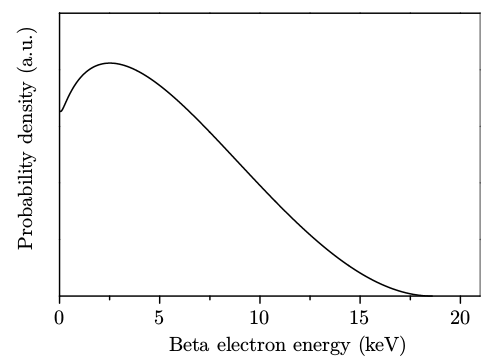
\includegraphics[scale=0.6]{Espectro.png}
\centering
\caption{Energy spectrum of tritium electrons ~\cite{TesisTritio}\label{fig:TritiumDecaySpectrum}}
\end{figure}


The releasing energy, which is produced in the tritium decay, is very little. In fact, it is the radioactive isotope with the lowest energy released in its $\beta$ disintegration \cite{dOCUMENTO MANIPULACIÓN SEGURA DEL TRITIO}. As a consequence the $\beta$ particles (electrons) which is emitted in this tritium decay is easily stopped. Indeed, we can see the mean free path of tritium electrons for several energies in the table \ref{MeanFreePathTritium}

\begin{table}[htbp]
\begin{center}
\begin{tabular}{|l|l|l|}
\hline
Material & Energy ($\beta$)(keV) & Penetration Depth \\
\hline \hline \hline
$\ce{\ce{^{3}_{1}H_2}}$, STP & 5.7 & 0.26 cm \\ \hline
$\ce{\ce{^{3}_{1}H_2}}$, STP & 18.6 & 3.2 cm \\ \hline
Air, STP & 5.7 & 0.036 cm \\ \hline
Air, STP & 18.6 & 0.45 cm \\ \hline
\parbox{10em}{\centering Water, soft tissue\\  (solid matter whose \\  density is $1~\gram\cdot\cm^{-3}$)} & 5.7 & 0.42 $\mu\meter$\\ \hline
\parbox{10em}{\centering Water, soft tissue\\  (solid matter whose \\  density is $1~\gram\cdot\cm^{-3}$)} & 18.6 & 5.2 $\mu\meter$ \\ \hline
\end{tabular}
\caption{Mean Free Path of tritium isotope for several energies~\cite{documento manipulación segura tritio}}
\label{MeanFreePathTritium}
\end{center}
\end{table}

JUSTIFICAR ESTOS RECORRIDOS LIBRES MEDIOS CON LOS CALCULOS TEÓRICOS HECHOS EN LA TESIS ALEMANA, PUNTO 3.1.

On the one hand, it means that the tritium electrons is easily stopped even for simply walls like our clothes or the laboratories gloves. The danger to health appears when we ingest or inhale tritium because their biologic life time (time during which tritium remains in our body) is between 7 and 14 days \cite{asdfass}, time during which we are receiving dose due to tritium radiation. Nowadays, there's exist several models with which we can calcule the dose which we have recived due to the introduccion of tritium in our body \cite{asdfasdf}. 

On the other hand, this short mean free path will be a problem when we try to detect tritium for several reasons which we will have to take into account when we design our detector if we want to overcome these: 

\begin{itemize}
\item{} Firstly, our radiactive source (tritium water) and the sensitive part of our detector (scintillating fibers in our case) have to be as close as posible (in contact in our case) because the activity of the radiation is exponentially attenuated and we have low activities so we cannot afford lose events. For this reason windows materials or fiber clads cannot be used because of the attenuation and because if it is thicker than $5\mu\meter$ we will lose practically all the signal.

\item{} Secondly, the active volume of our detector will be practically the active area to our detector so we need to design our detector with large active area (area or the scintilalting fibers with which we can detect tritium) and a thickness as small as possible (thickness of the scintillating fibers) because the part of the fiber with thickness bigger than the mean free path of tritium decay ($5-6 \mu\meter$ in low molecular weight solids) only will contribute to the system as background.

\item{} Thirdly, we have to take into account that this low energy of tritium decay will result in a low quantum efficiency in our detector.

\end{itemize}

In the tritium decay, equation \ref{TritiumDecay}, the existence of the antineutrino is imposed, among other things, by the conservation of the leptonic number, specifically the leptonic number of the electron family ($L_e$). In practice, we don't have the posssibility of detecting this particle because it interacts very weakly with matter and, therefore, with our detector ($\sigma \propto 10^{-42} ~ \cm^2$). That is, this particle escapes without interacting and instead, we only detect its absence, i mean, the non-preservation of certain physical quantities such as energy, momentum, leptonic number, etc. in the particles which we detect.

Therefore, for mesuring the tritium decay, we only have the possibility of detecting the stable isotope $\ce{^{3}He}$ or/and the electron. Keep in mind that, although the isotope son of the tritium decay reaction, $\ce{^{3}He}$, is stable, it is in a non-stationary state, that is, it is not in a self-state of its Hamiltonian, but in a state that can be expressed as a sum of self-states of the Hamiltonian. As a consequence, after the tritium $\beta^-$ decay, we will have a subsequent dexcitation of the $\ce{^{3}He}$ which will produce fotons with several well-defined energies that correspond to their energy levels, photons which we can observe in our detector.

In summary, we will obtain a tritium decay spectrum added to a typical X-ray spectrum of $\ce{^{3}He}$ which will have, ideally, several discrete values but, due to the non-zero uncertainty of our detectors, this spectrum will have several gaussians.

Furthermore, since $\ce{^{3}He}$ has a much higher mass than electrons and neutrinos, by conservation of energy and momentum, we can see that it will hardly move from the point where the reaction occurs. Therefore, we focus on electrons detection.



CAMBIAR LA REFERENCIA DE LA FOTO POR LA DEL TFG DE ANA
IMAGENES DE DESINTEGRACION DEL TRITIO (TFG ANA)

Resumer todo esto ultimo:

The 3He nucleus carries a very small fraction of the energy due to the conservation of momentum and its larlge mass. The electron-antineutrino (simbolo) reacts very rarely with matter (sección eficaz) therefore practically only the beta decay electron affects it surroundings. 

Tritium at normal temperature and pressure (273 K, 10 5 Pa) is a gas, forming two-atom
molecules, and having the same chemical properties as hydrogen. Due to its chemical
properties it can easily substitute hydrogen atoms in a water molecule, and form triti-
ated water (hereinafter also abbreviated as HTO 1 ). The beta radiation of tritium can
break up the water molecules (radiolysis), which then form radicals in the water. This
results in a corrosivity higher than that of non-tritiated water [39], [40].
Chemically, tritiated water molecules behave similar to normal water, therefore they
can also substitute normal water in the human body, which leads a high radiotoxicity of
tritiated water [21]. Therefore, it has to be specially handled (see next section).

Tritium at normal temperature and pressure (273 K, 10 5 Pa) is a gas, forming two-atom
molecules, and having the same chemical properties as hydrogen. Due to its chemical
properties it can easily substitute hydrogen atoms in a water molecule, and form triti-
ated water (hereinafter also abbreviated as HTO 1 ). The beta radiation of tritium can
break up the water molecules (radiolysis), which then form radicals in the water. This
results in a corrosivity higher than that of non-tritiated water [39], [40].
Chemically, tritiated water molecules behave similar to normal water, therefore they
can also substitute normal water in the human body, which leads a high radiotoxicity of
tritiated water [21]. Therefore, it has to be specially handled (see next section).

Pure tritiated water (without hydrogen or deuterium in the water molecules) of course contains T 2 O molecules, but this form is produced only in special experiments. Tritiated water in the concentration range of water detritiation facilities (some kBq/l to several GBq/l) contains some ppm tritium, and since the tritium atoms are evenly distributed among the water molecules in equilibrium, most
tritiated molecules are HTO.

Tritio es igual quimicamente pero diferente nuclearmente al hidrogeno. Documento de manipulación segura del tritio. alomejor incluir la tabla 2.

El rango del tritio hace que no sea peligroso pero presenta problemas de detección. Donde otros isotopos son faciles de detectar gracias a su poder de penetración el tritio tiene que ser introducido directamente dentro del detector para ser medido.




"Comparative study of pre-treatment procedures for 3H monitoring in water samples from environmental protection programs":
- Intro, basada en la referencia 8 de la tesis alemana. Interesante dar estas cantidades.

-Punto 2.1- Tipicos elementos radiactivos que poseen las muestras en la naturaleza. Complementarlo con los librillos del LARAM.




Pure tritiated water (without hydrogen or deuterium in the water molecules) of course contains T 2 O molecules, but this form is produced only in special experiments. Tritiated water in the concentration range of water detritiation facilities (some kBq/l to several GBq/l) contains some ppm tritium, and since the tritium atoms are evenly distributed among the water molecules in equilibrium, most tritiated molecules are HTO.

Tritium at normal temperature and pressure (273 K, 10 5 Pa) is a gas, forming two-atom
molecules, and having the same chemical properties as hydrogen. Due to its chemical
properties it can easily substitute hydrogen atoms in a water molecule, and form triti-
ated water (hereinafter also abbreviated as HTO 1 ). The beta radiation of tritium can
break up the water molecules (radiolysis), which then form radicals in the water. This
results in a corrosivity higher than that of non-tritiated water [39], [40].
Chemically, tritiated water molecules behave similar to normal water, therefore they
can also substitute normal water in the human body, which leads a high radiotoxicity of
tritiated water [21]. Therefore, it has to be specially handled (see next section).


 

TODO LO DE ARRIBA ES COPIADO DE LA TESIS ALEMANA.

Although isotopes of an element hagve almost the same chemical properties, the nuclear properties can be quite different. -> PREMIER DE MANIPULACION SEGURA DE TRITIUM DOE
Incluir tambien la tabla 1

referencia 39 de la tesis alemana: 
-la ecuación de la desintegración del tritio es tal. En el caso de moleculas es... formulas 3 y 4.
-Furthermore, the energy of E particles formed
through tritium radioactive decay (E max = 18.6 keV,
E average = 5.7 keV) is enough to break hydrogen – oxygen
bonds in water molecules (E bond = 5.2 eV) or to ionise
water (E ion = 12.6 eV). The interaction between E
particles and water molecules initiates water
decomposition through the phenomenon called self-
radiolysis.
